\documentclass{anstrans}
%%%%%%%%%%%%%%%%%%%%%%%%%%%%%%%%%%%
\title{Eddington Acceleration}
\author{Samuel S. Olivier*}

\institute{Department of Nuclear Engineering, Texas A\&M University, College Station, TX 77843}

\email{smsolivier@tamu.edu}


%%%% packages and definitions (optional)
\usepackage{graphicx} % allows inclusion of graphics
\usepackage{booktabs} % nice rules (thick lines) for tables
\usepackage{microtype} % improves typography for PDF

\usepackage{xspace}
\usepackage{siunitx}

\newcommand{\SN}{S$_N$\xspace}
\renewcommand{\vec}[1]{\bm{#1}} %vector is bold italic
\newcommand{\vd}{\bm{\cdot}} % slightly bold vector dot
\newcommand{\grad}{\vec{\nabla}} % gradient
\newcommand{\ud}{\mathop{}\!\mathrm{d}} % upright derivative symbol
\newcommand{\pderiv}[2]{\frac{\partial #1}{\partial #2}}
\newcommand{\dderiv}[2]{\frac{\ud #1}{\ud #2}}
\newcommand{\edd}{\langle \mu^2 \rangle} 

% add section on MHFEM system 
% order of accuracy of accelerated system 

\begin{document}
\section{Introduction}
	One of the most challenging computational tasks is to simulate the interaction of radiation with matter. The steady--state, one--group, isotropically--scattering, fixed--source Linear Boltzmann Equation in planar geometry is: 
		\begin{equation} \label{eq:bte}
			\mu \pderiv{\psi}{x}(x, \mu) + \Sigma_t(x) \psi(x,\mu) = 
			\frac{\Sigma_s(x)}{2} \int_{-1}^{1} \psi(x, \mu') d\mu' + \frac{Q(x)}{2}
		\end{equation}
	where $\mu = \cos\theta$ is the cosine of the angle of flight $\theta$ relative to the $x$--axis, $\Sigma_t(x)$ and $\Sigma_s(x)$ the total and scattering cross sections, $Q(x)$ the isotropic fixed--source and $\psi(x, \mu)$ the angular flux \cite{adams}. In the Discrete--Ordinates (\SN) angular discretization, $\mu$ takes values from Gauss Legendre quadrature. The scalar flux, $\phi(x)$, is then 
		\begin{equation} \label{eq:quad}
			\phi(x) = \int_{-1}^1 \psi(x, \mu) \ud\mu 
				\xrightarrow{\text{S}_N} \sum_{n=1}^N w_n \psi_n(x)
		\end{equation}
	where $\psi_n(x) = \psi(x,\mu_n)$ and $w_n$ the quadrature weights corresponding to each $\mu_n$ \cite{llnl}. The \SN equations are then 
		\begin{equation} \label{eq:sn}
			\mu_n \dderiv{\psi_n}{x}(x) + \Sigma_t(x) \psi_n(x) = 
			\frac{\Sigma_s(x)}{2} \sum_{n=1}^N w_n \psi_n(x) + \frac{Q(x)}{2} 
		\end{equation}
	for $n = 1, 2, \dots, N$. 

	In the Source Iteration (SI) scheme, the right hand side of Eq. \ref{eq:sn} is lagged. In other words, 
		\begin{equation} \label{eq:si}
			\mu_n \dderiv{\psi_n^{\ell+1}}{x}(x) + \Sigma_t(x) \psi_n^{\ell+1}(x) = 
			\frac{\Sigma_s(x)}{2} \sum_{n=1}^N w_n \psi_n^\ell(x) + \frac{Q(x)}{2}. 
		\end{equation}
	Equation \ref{eq:si} is iterated until the flux converges. If $\phi^0(x) = 0$ then $\phi^\ell$ is the scalar flux of particles that have undergone $\ell - 1$ collisions \cite{adams}. Thus, the number of iterations until convergence is directly linked to the number of collisions in a particle's lifetime. Typically, SI becomes increasingly slow to converge as the ratio of $\Sigma_s$ to $\Sigma_t$ approaches unity. 

	Fortunately, the regime where SI is slow to converge is also the regime where Diffusion Theory is most accurate. A popular method for accelerating SI is Diffusion Synthetic Acceleration (DSA) where a transport sweep is conducted and then a diffusion solve is used to generate a correction factor. DSA requires correction schemes such as the Source Correction, Diffusion Coefficient, and Removal Correction schemes presented in \cite{alcouffe} to prevent instability in highly scattering regimes with coarse spatial grids. 

	Lawrence Livermore National Laboratory (LLNL) is developing a high--order radiation--hydrodynamics code. The hydrodynamics portion is discretized using the Mixed--Hybrid Finite Element Method (MHFEM), where values are taken to be constant within a cell with discontinuous jumps at both cell edges \cite{mhfem}. MHFEM is particularly suited for hydrodynamics but not for radiation transport. This work seeks to efficiently accelerate \SN calculations with a scheme that is both robust and compatible with MHFEM hydrodynamics. 

\section{Eddington Acceleration}
	The zeroth and first angular moments of Eq. \ref{eq:bte} are 
		\begin{subequations} 
		\begin{equation} \label{eq:zero}
			\dderiv{}{x} J(x) + \Sigma_a(x) \phi(x) = Q(x) 
		\end{equation} 
		\begin{equation} \label{eq:first}
			\frac{\ud}{\ud x} \edd(x) \phi(x) + \Sigma_t J = 0  
		\end{equation}
		\end{subequations}
	where $J = \int_{-1}^{1} \mu \ \psi(x, \mu) \ud \mu$ is the current and 
		\begin{equation} \label{eq:eddington} 
			\edd(x) = \frac{\int_{-1}^1 \mu^2 \psi(x, \mu) \ud \mu}{\int_{-1}^1 \psi(x, \mu) \ud \mu}
		\end{equation}
	the Eddington factor. When $\edd(x) = \frac{1}{3}$, Eqs. \ref{eq:zero} and \ref{eq:first} are equivalent to Diffusion Theory. 

	The proposed acceleration scheme is: 
		\begin{enumerate}
			\item Compute $\psi_n$ with \SN and an arbitrary spatial discretization
			\item Compute $\edd$ 
			\item Interpolate $\edd$ onto the MHFEM grid 
			\item Solve the moment equations with the preconditioned $\edd$ using MHFEM. 
		\end{enumerate}
	This scheme allows the \SN equations and moment equations to be solved with different spatial discretizations. This means \SN can be discretized using normal methods such as Linear Discontinuous Galerkin or Diamond Differencing while the moment equations can be solved on the same grid as the hydrodynamics. 

	This method differs from DSA in that two solutions are generated: one from \SN and one from the moment equations and that the \SN and acceleration steps do not have to be consistently differenced. The solution of the moment equations will be used because the moment equations are conservative while \SN is not. 
\section{Results}
	As a proof of concept for Eddington acceleration, a Diamond Differenced \SN code was created in addition to an MHFEM solver for Eqs. \ref{eq:zero} and \ref{eq:first}. The test problem of steady--state, one--group, isotropically--scattering, fixed--source radiation transport in slab geometry with a reflecting left boundary and vacuum right boundary was used to compare unaccelerated, Eddington accelerated and DSA S$_8$ with 100 spatial cells. Figure \ref{fig:comparison} shows the number of iterations until the L$^2$ norm of the flux converged to within a tolerance of \num{1e-6} for varying ratios of $\Sigma_s$ to $\Sigma_t$. 


	\begin{figure}[ht] % replace 't' with 'b' to force it to be on the bottom
	  \centering
	  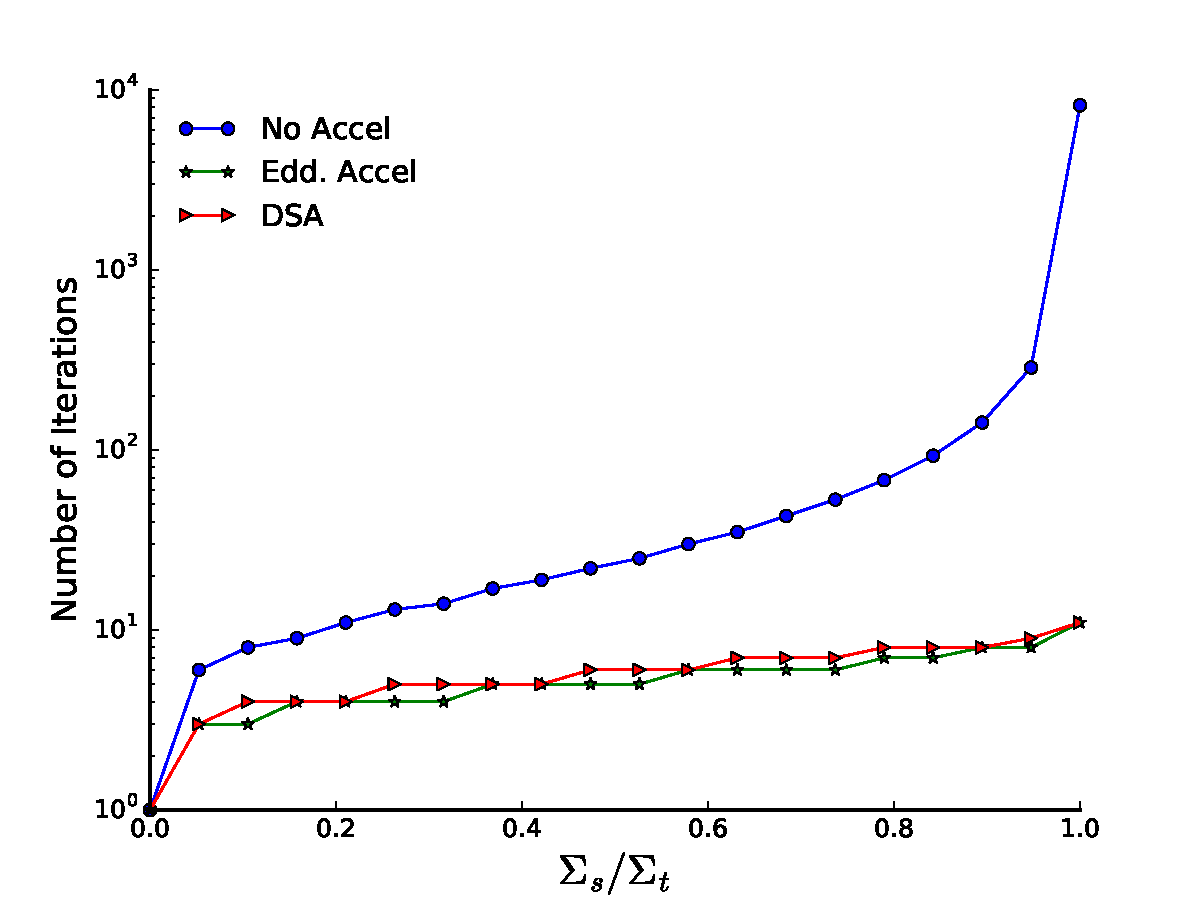
\includegraphics[width=8.5cm]{accel.pdf}
	  \caption{A comparison of unaccelerated, Eddington accelerated and DSA S$_8$. }
	  \label{fig:comparison}
	\end{figure}

\section{Conclusions}
	Figure \ref{fig:comparison} suggests that Eddington acceleration is a valid method for accelerating \SN SI calculations. The required iterations until convergence is significantly lower for Eddington accelerated S$_8$. This is especially evident for the pure scattering regime ($\Sigma_s = \Sigma_t$) where S$_8$ was accelerated by a factor of 750. In addition, Eddington acceleration performed as well as DSA. This scheme produces a conservative solution and does not require the \SN and acceleration steps to be consistently differenced. 

\section{Future Work} 
	

\section{Acknowledgments}

\bibliographystyle{ans}
\bibliography{bibliography.bib}
\end{document}